\documentclass{beamer}
\usepackage[utf8]{inputenc}
\usepackage{graphicx}
\usepackage{fancyvrb}
\usepackage{eurosym}
\usepackage{xcolor}
\usepackage{textcomp}
\usepackage[ruled, lined]{algorithm2e}
\usepackage{tikz}
\usepackage{multirow}
\usepackage{booktabs}
\usetheme{simple}

\let\Tiny=\tiny

\newcommand{\mytilde}{$\sim$}

\definecolor{links}{HTML}{2A1B81}
\hypersetup{colorlinks,linkcolor=,urlcolor=links}

\addtolength{\jot}{0.6em}  % extra space between align rows
\DeclareUnicodeCharacter{20AC}{\euro}

\newenvironment{wideitemize}{\itemize\addtolength{\itemsep}{10pt}}{\enditemize}
\newenvironment{wideenumerate}{\enumerate\addtolength{\itemsep}{8pt}}{\endenumerate}

\usetikzlibrary{arrows,shapes,positioning}
\graphicspath{{img/}}

\title{Introducción a R}
\author{Alberto Torres Barrán}
%\institute[UAH]{Universidad de Alcalá de Henares}
\date{22 de Mayo de 2018}

\begin{document}
\begin{frame}[plain]
\titlepage
\end{frame}

\begin{frame}[allowframebreaks]
	\frametitle{Índice}
    \tableofcontents[sections={1-4}]
      \framebreak
    \tableofcontents[sections={5-9}]
\end{frame}

% \AtBeginSection[]
% {
%    \begin{frame}
%        \frametitle{Índice}
%        \tableofcontents[currentsection]
%    \end{frame}
% }

\section{Introducción}

\begin{frame}
\frametitle{Introducción}

% motivacion!!
\begin{itemize}
\item R es un lenguaje de programación y un entorno para manipular datos, cálculo y gráficos.
\item Ventajas:
\begin{itemize}
\item Proyecto de GNU (\textit{open source}), cualquier puede contribuir al desarrollo.
\item Gran cantidad de paquetes (12585 a 21 de Mayo de 2018).
\item La mayoría de nuevas tecnologías y algoritmos relacionados con estadística aparecen primero en R.
\item Documentación abundante en Internet, muchos grupos de usuarios activos.
\end{itemize}
\item Desventajas:
\begin{itemize}
\item Curva de aprendizaje inclinada, como la mayoría de lenguajes de programación.
\item Menor rendimiento que otros lenguajes de cálculo científico.
\item Gestión de memoria.
\end{itemize}
\end{itemize}

\end{frame}

\begin{frame}[fragile]
\frametitle{Comparación rendimiento}
\begin{center}
\begin{tabular}{lrrrrrrr}
\toprule
&Fortran&Python&R&Matlab&Java \\
\midrule
fib&0.57&95.45&528.85&4258.12&0.96 \\
parse\_int&4.67&20.48&54.30&1525.88&5.43 \\
quicksort&1.10&46.70&248.28&55.87&1.65 \\
mandel&0.87&18.83&58.97&60.09&0.68 \\
pi\_sum&0.83&21.07&14.45&1.28&1.00 \\
rand\_mat\_stat&0.99&22.29&16.88&9.82&4.01 \\
rand\_mat\_mul&4.05&1.08&1.63&1.12&2.35 \\
\bottomrule
\end{tabular}
\vspace*{1em}

Tiempos de benchmark relativos a C (más pequeño es mejor, rendimiento de C = 1.0). Fuente: \url{http://julialang.org/}
\end{center}
\end{frame}

\begin{frame}
\frametitle{Entorno R}

\begin{itemize}
\item R es un lenguaje interpretado, por lo que no es necesario compilar el código fuente.
\item El intérprete de R está disponible para los principales sistemas operativos (Windows, OSX y Linux): \url{http://cran.r-project.org}.
\item En este curso vamos a trabajar con el IDE RStudio \url{http://www.rstudio.com}.
\item RStudio proporciona un entorno similar al de Matlab.
\item Documentación y manuales: \url{http://www.r-project.org}.
\end{itemize}
\end{frame}

\begin{frame}[fragile]
\frametitle{Comandos de R}

\begin{itemize}
\item Distinguen entre mayúsculas y minúsculas.
\item Se clasifican en \textit{asignaciones} (el resultado se guarda) y \textit{expresiones} (el resultado se imprime y se pierde).
\item El operador de asignación es \texttt{<-} o \texttt{->} (no \texttt{=}, como en la mayoría de lenguajes).
\item Los comandos se pueden escribir de forma interactiva en el intérprete o almacenar en un fichero de texto.
%\item Un fichero de comandos se carga con la expresión \verb+   > source("fichero.R")+
\item Para obtener ayuda sobre un determinado comando se utiliza la expresión \\ \verb+   > help("lm")+ \\o alternativamente \\ \verb+   > ?lm+
\end{itemize}
\end{frame}

\begin{frame}[fragile]
\frametitle{Scripts de R}
\begin{itemize}
\item Si se re-utilizan secuencias de comandos con frecuencia, es conveniente guardarlas en un fichero \texttt{script.R}.
\item El fichero se puede ejecutar posteriormente en R con
\begin{verbatim}
   > source("script.R")
\end{verbatim}
\item El intérprete de R ejecutará cada una de las líneas del fichero, pero sin imprimir el valor de ninguna variable en la consola.
\item Para ello, son útiles las funciones \texttt{cat()} y \texttt{print()}, que imprimen por pantalla el valor de las variables pasadas como argumentos.
\item Es importante destacar que el fichero \texttt{script.R} tiene que estar en el directorio de trabajo actual, de lo contrario hay que usar la ruta completa.
\end{itemize}
\end{frame}

\section{Objetos}

\begin{frame}[fragile]
\frametitle{Objetos}

\begin{itemize}
\item Todas las entidades que R manipula se denominan objetos (variables, funciones, etc).
\item Para crear un objeto se utiliza el operador de asignación.
\item Los objetos se almacenan en la memoria RAM del ordenador con un nombre específico.
\item Para cambiar el valor de un objeto hay que asignarlo de nuevo.
\item Listar todos los objetos en memoria \\ \verb+   > ls()+
\item Eliminar objetos \texttt{x} y \texttt{tmp} de la memoria \\ \verb+   > rm(x, tmp)+
\item Al cerrar la sesión se pueden almacenar todos los objetos en el fichero \texttt{.RData}.
\item Al abrir una nueva sesión se cargaran los objetos del fichero \texttt{.RData} almacenado en el directorio actual (si existe).
\end{itemize}

\end{frame}

% DEMO time!!
% Abrir el intérprete de Windows, Linux, RStudio y enseñar la distinta funcionalidad.
% Crear un par de asignaciones y expresiones, ver la ayuda
% Orientado a objetos: todas las variables, resultados, datos (objetos) se almacenan en la memoria
% Como crear y destruir objetos.
% Ver los objetos.

\begin{frame}[fragile]
\frametitle{Objetos (cont.)}
\begin{itemize}
\item Los tipos de datos básicos son \texttt{numeric}, \texttt{complex}, \texttt{logical} y \texttt{character}.
\item El modo de un objeto es el tipo básico de los elementos que contiene, se puede ver con la función \texttt{mode()}.
\item Para convertir de un modo a otro se utilizan las funciones \verb+as.character()+, \verb+as.numeric()+, etc.
\item Todos los objetos tienen una clase, que se puede ver con la función \texttt{class()}.
\item Algunas funciones producirán un resultado u otro dependiendo de la clase de sus argumentos.
\item Las funciones \verb+is.character()+, \verb+is.numeric()+, etc. devuelven verdadero o falso dependiendo si el objeto es de esa clase o no.
\end{itemize}
\end{frame}

\begin{frame}
\frametitle{Funciones}

\begin{itemize}

\item Las funciones son un tipo especial de objetos.

\item Dados unos argumentos o parámetros de entrada, realizan una operación sobre los mismos y devuelven un resultado.

\item En ocasiones también tienen parámetros opcionales.

\item En general las funciones no modifican el valor de sus argumentos.

\item Los parámetros de entrada tienen que ser de una clase o clases determinadas por la propia función.

\item En la ayuda se puede ver el número y clase de cada uno de los parámetros que acepta junto con información detallada acerca de la función.
\end{itemize}
\end{frame}

% razon por la que existe el tipo integer, double o single (para pasar a C y Fortran)
% de hecho, los enteros se representan como numeric

% en R todo es un vector!!!

\section{Estructuras de datos básicas: vector, array, list}

\begin{frame}
\frametitle{Vectores}
\begin{wideitemize}
\item Un vector es una secuencia de datos del mismo tipo básico.
\item Creación de vectores:
\begin{enumerate}
\item Función \texttt{c()}: combina sus argumentos para formar un vector, intenta convertirlos al mismo tipo (si es posible).
\item Función \texttt{vector()}: tiene dos argumentos, el \texttt{tipo} y la \texttt{longitud}.
\item Funciones \texttt{numeric()}, \texttt{integer()}, etc.: igual que \texttt{vector()} pero tienen un único argumento, que es la longitud del vector.
\end{enumerate}
\item Para ver la longitud de un vector se utiliza \texttt{length()}.
\end{wideitemize}
\end{frame}

\begin{frame}
\frametitle{Aritmética vectorial}

\begin{itemize}
\item Los siguientes expresiones se pueden aplicar en vectores:
\begin{itemize}
\item Operadores aritméticos: \texttt{+}, \texttt{-}, \texttt{*}, \texttt{/}, \texttt{\^}, \texttt{\%\%} y \texttt{\%/\%}.
\item Funciones: \texttt{log}, \texttt{exp}, \texttt{sin}, \texttt{cos}, \texttt{tan} y \texttt{sqrt}.
\item Operadores lógicos: \texttt{\&}, \texttt{!} y \texttt{|}.
\end{itemize}
\item Realizan las operaciones elemento a elemento.
\item Los vectores pueden ser de distintas longitudes: los vectores más cortos reciclan sus elementos hasta tener la longitud del más largo.
\item Otras funciones que operan sobre vectores (no elemento a elemento): \texttt{sum()}, \texttt{prod()}, \texttt{max()}, \texttt{min()}, \texttt{range()}, \texttt{mean()}, \texttt{var()}, \texttt{sd()}, \texttt{cumsum()}, \texttt{cumprod()}, etc...
\end{itemize}
\end{frame}

\begin{frame}[fragile]
\frametitle{Sucesiones}

\begin{wideitemize}
\item Operador ``\texttt{:}''. Genera números enteros en un rango, tiene máxima prioridad. \\ \verb+   > 1:20+
\item Función \texttt{seq()}. Genera secuencias más complejas. Por ejemplo:
\begin{verbatim}
   > seq(-0.5, 0.5, by=.2)
    [1] -0.5 -0.3 -0.1  0.1  0.3  0.5
\end{verbatim}
\item Función \texttt{rep()}. Duplica el objeto. Ejemplos:
\begin{verbatim}
   > rep(1, 10)
    [1] 1 1 1 1 1 1 1 1 1 1
   > rep(1:4, 2)
    [1] 1 2 3 4 1 2 3 4
\end{verbatim}
\end{wideitemize}
\end{frame}

%% Funciones para cadenas de caracteres (paste!) con varios vectores parecido a zip de numpy

\begin{frame}[fragile]
\frametitle{Selección de subvectores}
\begin{itemize}
\item Para seleccionar partes de un vector se utilizan vectores de índices entre corchetes \texttt{[} y \texttt{]}.
\item Hay 4 tipos de vectores de índices:
\begin{enumerate}
\item Vector lógico: se seleccionan los valores que son \texttt{TRUE}.
\item Vector de enteros positivos: se seleccionan los elementos con esos índices.
\item Vector de enteros negativos: se excluyen los elementos con esos índices.
\item Vector de caracteres: solo si los elementos del vector tienen nombre, selecciona los elementos con dicho nombre.
\end{enumerate}
\item La variable de almacenamiento también puede ser indexada.
\item Poner a 0 los elementos de \texttt{x} menores que 5:
\begin{verbatim}
   > x[x < 5] <- 0
\end{verbatim}
\end{itemize}
\end{frame}

\begin{frame}[allowframebreaks, fragile]
\frametitle{Ejercicio}

Ejecutar el siguiente código en R, que genera dos vectores de enteros aleatorios elegidos entre el 1 y el 1000 de tamaño 250:
\begin{verbatim}
   > n <- 250
   > x <- sample(1:1000, n, replace=T)
   > y <- sample(1:1000, n, replace=T)
\end{verbatim}

A partir de los dos vectores anteriores:

\begin{wideenumerate}
\item Calcular el el máximo y el mínimo de los vectores $x$ e $y$.
\item Calcular la media de los vectores $x$ e $y$. Antes de calcularla, ¿que valor esperarías?.
\item Calcula el número de elementos de $x$ divisibles por 2 (el operador módulo es \texttt{\%\%}).
\framebreak
\item Ordenar los vectores, primero usando la función \texttt{order()} y luego la función \texttt{sort()}.
\item Seleccionar los valores de $y$ menores que $600$.
\item Crear las secuencias (funciones \texttt{rep} y \texttt{seq}):
\begin{itemize}
\item \texttt{1 2 3 4 5 6 7 8 9 10}.
\item \texttt{1 2 3 4 1 2 3 4 1 2 3 4}.
\item \texttt{-1 -0.8 -0.6 -0.4 -0.2 0 0.2 0.4 0.8 1}.
\end{itemize}
%\item Crear el vector $$(x_1+2x_2-x_3,\ x_2+2x_3-x_4 , . . . ,\ x_{n-2}+2x_{n-1}-x_{n})$$ \textbf{Pista}: tiene tamaño $n-2$.
\end{wideenumerate}
\end{frame}


\begin{frame}[fragile]
\frametitle{Arrays}
\begin{wideitemize}
\item Un \texttt{array} es una colección de datos del mismo tipo indexada por varios índices.
\item La función \texttt{dim()} devuelve la longitud de cada una de las dimensiones del \texttt{array}.
%\item Un vector se puede transformar en un \texttt{array} modificando su atributo \textit{dim}:
%\begin{verbatim}
%   > x <- 1:60
%   > dim(x) <- c(3,5,4)
%\end{verbatim}
\item Los \texttt{arrays} se crean con la función \texttt{array()} y sus datos se rellenan con el primer índice variando más rápido:
\begin{verbatim}
   > z <- array(x, dim=c(3,5,4))
\end{verbatim}
%\item La diferencia entre los métodos anteriores es que el primero evita duplicar el objeto.
\end{wideitemize}
\end{frame}

\begin{frame}[fragile, allowframebreaks]
\frametitle{Selección de subarrays}

\begin{wideitemize}
\item En general, se puede seleccionar una parte del \texttt{array} mediante una sucesión de vectores índice.
\begin{verbatim}
   > z[1:2, -(1:4), 2]
   [1] 28 29
\end{verbatim}
\item Si un vector índice está vacio se selecciona todo el rango de valores.
\begin{verbatim}
   > z [,,1]
      [,1] [,2] [,3] [,4] [,5]
   [1,]    1    4    7   10   13
   [2,]    2    5    8   11   14
   [3,]    3    6    9   12   15
\end{verbatim}
%\framebreak
%\item Los arrays también se pueden indexar con otro array de índices.
%\item En el siguiente ejemplo, estamos seleccionando los elementos \texttt{z[1,1,3]} y \texttt{z[2,2,1]}
%\begin{verbatim}
%   > idx <- array(c(1:2, 1:3), dim=c(2,3))
%   > idx
%        [,1] [,2] [,3]
%   [1,]    1    1    3
%   [2,]    2    2    1
%   > z[idx]
%   [1] 31  5
%\end{verbatim}
\end{wideitemize}
\end{frame}


\begin{frame}
\frametitle{Matrices}
\begin{itemize}
\item Una \texttt{matriz} es un \texttt{array} de 2 dimensiones.
\item Las matrices se crean con la función \texttt{matrix()}, y sus datos se rellenan por columnas (igual que en los arrays).
\item Las funciones \texttt{nrow()}, \texttt{ncol()} devuelven el número de filas y columnas de forma respectiva.
\item Además de todos los operadores de arrays, existen funciones específicas para matrices:
\begin{description}
\item[\texttt{t()}] devuelve la transpuesta de una matriz.
\item[\texttt{diag()}] devuelve la diagonal de una matriz.
\item[\texttt{crossprod()}] realiza el producto cruzado entre matrices (equivalente al operador \texttt{\%*\%}).
\item[\texttt{eigen()}] calcula autovalores y autovectores.
\item[\texttt{svd()}] realiza la descomposición en valores singulares.
\end{description}
\end{itemize}
\end{frame}


\begin{frame}[allowframebreaks]
\frametitle{Ejercicio matrices}
\begin{enumerate}
\item Crear la matriz $4 \times 5$, $$A = \begin{pmatrix} 1 & 2 & 3 & 4 & 5 \\ 6 & 7 & 8 & 9 & 10 \\ 11 & 12 & 13 & 14 & 15 \\ 16 & 17 & 18 & 19 & 20 \end{pmatrix}$$ \textbf{Pista}: ver el parámetro \texttt{byrow} de la función \texttt{matrix()}.

\item Extraer los elementos $A[4,3], A[3,4], A[2,5]$ utilizando una matriz de índices.

\item Reemplazar dichos elementos con $0$.
\framebreak
\item Crear la matriz identidad $5 \times 5$, $$\mathbf{I} = \begin{pmatrix} 1 & 0 & \dots & 0 \\ 0 & 1 & \dots & 0 \\ \vdots & \vdots & \ddots & \vdots \\ 0 & 0 & \dots & 1 \end{pmatrix}$$ \textbf{Pista}: mirar documentación de la función \texttt{diag()}.
\item Convertir la matriz $A$ anterior en una matriz cuadrada $B$ añadiendo al final una fila de unos (función \texttt{rbind()}): $$B = \begin{pmatrix} A \\ \mathbf{1} \end{pmatrix}$$
\item Calcular la inversa de la matriz $B$ con la función \texttt{solve()}.
\framebreak
\item Multiplicar $B$ por su inversa $B^{-1}$.
\item Comprobar si el resultado es exactamente la matriz identidad $\mathbf{I}$.
\item En caso contrario, calcular el ``error'' o ``precisión'' de la operación, definido como: $$\text{Error} = \frac{1}{N}\sum_{i,j}{|(BB^{-1} - \mathbf{I})_{(i,j)}|}$$ donde $N$ es el número de elementos de la matriz $B$.
\end{enumerate}
\end{frame}


\begin{frame}[fragile]
\frametitle{Listas}

\begin{itemize}
\item Una lista consiste en una colección ordenada de objetos del mismo o distinto tipo.
\item Los componentes de la lista siempre están numerados.
\item Son accesibles con el operador doble corchete \texttt{[[} y \texttt{]]}:
\begin{verbatim}
   > l <- list(nombre="Alberto", numeros=c(3,5,6))
   > l[[1]]
   [1] "Alberto"
\end{verbatim}
\item Los componentes también pueden tener nombre. En ese caso también son accesibles de la siguiente forma:
\begin{verbatim}
   > l$nombre
   [1] "Alberto"
   > l[["numeros"]]
   [1] 3 5 6
\end{verbatim}
\end{itemize}
\end{frame}

\begin{frame}[fragile]
\frametitle{Operaciones sobre listas}
\begin{itemize}
\item Se crean con la función \texttt{list()}.
\item Se pueden modificar sus elementos con la sintaxis:
\begin{verbatim}
   > l$nombre <- "Juan"
\end{verbatim}
\item Si el nombre del elemento no existe, se añade a la lista:
\begin{verbatim}
   > l$edad <- 25
\end{verbatim}
\item También se pueden combinar con la función \texttt{c()} (similar a como se hacía con vectores).
\item Importante destacar la diferencia entre \texttt{l[[1]]} y \texttt{l[1]}: el primero devuelve el componente mientras que el segundo devuelve una sublista.
\end{itemize}
\end{frame}


\section{Estructuras de datos derivadas: data.frame, factor}

\begin{frame}[fragile]
\frametitle{Factores}
\begin{itemize}
\item Un factor es un tipo de dato que se utiliza para codificar valores categóricos, por ejemplo: \texttt{renta} = \{alta, baja, media\}.
\item Se crean con la función factor:
\begin{verbatim}
   > f <- factor(c("hombre", "mujer", "mujer"))
\end{verbatim}
\item Se pueden ver los niveles (valores distintos) con la función \texttt{levels()}:
\begin{verbatim}
   > levels(f)
   [1] "hombre" "mujer"
\end{verbatim}
\item Función \texttt{relevel()}: reordena los niveles del factor especificado, poniendo el nivel especificado de primero
\end{itemize}
\end{frame}

\begin{frame}
  \frametitle{Operaciones con factores}
  \begin{itemize}
    \item Función \texttt{cut()}: crea un factor dividiendo en rangos un vector numérico de acuerdo a unos puntos de corte
    \item Función \texttt{tapply()}: aplica una función a cada uno de los elementos de un vector, dividos en los distintos grupos de un determinado factor.
    \item Función \texttt{by()}: similar a la anterior, pero el objeto sobre el que se aplica la operación agrupada puede ser un \texttt{data.frame}.
    \item Función \texttt{aggregate()}: similar a \texttt{tapply()} pero devuelve un \texttt{data.frame} y acepta ``fórmulas''.
    \item Funciones \texttt{table()}, \texttt{prop.table()}, \texttt{margin.table()} y \texttt{xtabs()}: crear tablas de contingencia a partir de ciertos factores
  \end{itemize}
\end{frame}

%\begin{frame}
%\frametitle{Operaciones con cadenas de caracteres}
%\begin{itemize}
%\item Para variables que tienen un número muy alto de valores distintos es mejor utilizar vectores de cadenas de caracteres.
%
%\item R no es un lenguaje especialmente diseñado para trabajar con cadenas de caracteres, pero existen funciones para realizar operaciones básicas:
%
%\begin{itemize}
%\item \texttt{substr(x, start, stop)}. Extrae subcadena de \texttt{x} entre las posiciones \texttt{start} y \texttt{stop}.
%\item \texttt{grep(pattern, x)}. Devuelve las posiciones del vector \texttt{x} donde se cumple la expresión regular \texttt{pattern}.
%\item \texttt{gsub(pattern, replacement, x)}. Reemplaza \texttt{pattern} por \texttt{replacement} en todas las cadenas del vector \texttt{x}.
%\end{itemize}
%\item Más información sobre expresiones regulares: \href{http://stat.ethz.ch/R-manual/R-patched/library/base/html/regex.html}{regex}.
%\end{itemize}
%\end{frame}


%\begin{frame}[fragile]
%\frametitle{Fórmulas}
%\begin{itemize}
%\item Las fórmulas son objetos especiales de R que respresentan relaciones simbólicas entre variables:
%
%\texttt{respuesta \mytilde\  variables independientes}
%
%\item Se usan en funciones como \texttt{aggregate()}, \texttt{boxplot()}, y \texttt{lm()}.
%
%\item Los operadores aritméticos tienen otro significado cuando se usan dentro de las fórmulas. Ejemplos:
%
%\begin{Verbatim}[commandchars=\\\{\}]
%   y \mytilde u + v + w + u:v + u:w + v:w
%   y \mytilde u * v * w - u:v:w
%   y \mytilde (u + v + w)^2
%\end{Verbatim}
%
%\item Si queremos que tengan su significado habitual tenemos que utilizar el operador \texttt{I()}:
%\begin{Verbatim}[commandchars=\\\{\}]
%   y \mytilde u + v + w + I(u*v) + I(u*w) + I(v*w)
%\end{Verbatim}
%\end{itemize}
%\end{frame}

\begin{frame}
\frametitle{Data frames}
\begin{itemize}
\item Un data frame es una lista donde cada uno de sus elementos se conocen como variables.
\item Además, tiene las siguientes restricciones:
\begin{itemize}
\item Los componentes deben de ser vectores, factores, matrices, listas u otros data frames.
\item Las matrices, listas y data frames contribuyen al nuevo data frame con tantas variables como columnas, elementos o variables tengan.
\item Los vectores no numéricos se transforman en factores.
\item Todos los vectores tienen que tener la misma longitud y las matrices el mismo número de filas.
\end{itemize}
\item Resumiendo, un data frame es como una matriz donde sus columnas pueden ser de tipos diferentes.
\end{itemize}
\end{frame}

\begin{frame}[fragile, allowframebreaks]
\frametitle{Operaciones con data.frames}

\begin{itemize}
\item Por su condición de listas, se puede acceder a cada una de las variables del data frame de las siguientes formas:
\begin{verbatim}
   > mtcars[[1]]
   > mtcars[["mpg"]]
   > mtcars$mpg
\end{verbatim}
\item El resultado es un vector del mismo tipo que el elemento del data frame.
\item Para obtener un subconjunto de las columnas se pueden indexar numéricamente o por nombre:
\begin{verbatim}
   > mtcars[1]
   > mtcars["mpg"]
\end{verbatim}
\item Al igual que en las listas, el resultado de las operaciones anteriores es otro data frame.
\framebreak
\item Para obtener un subconjunto de las filas se pueden indexar numéricamente, por el nombre o usando un vector lógico:
\begin{verbatim}
   > mtcars[1,]
   > mtcars["Camaro Z28",]
   > mtcars[mtcars$mpg > 30,]
\end{verbatim}
\item Por último, se pueden combinar las dos anteriores para acceder a un subconjunto de las filas y de las columnas:
\begin{verbatim}
   > mtcars[4:8, -c(5:11)]
   > mtcars["Camaro Z28", c("mpg", "gear")]
   > mtcars[mtcars$mpg > 30, c(1,4)]
\end{verbatim}
\item El resultado de la operación es otro data frame, menos si es un único elemento ó se seleccionan todas las filas:
\begin{verbatim}
   > mtcars[,1]
\end{verbatim}
\end{itemize}
\end{frame}

%\begin{frame}[fragile]
%\frametitle{Funciones attach, detach y search}
%\begin{itemize}
%\item La notación para acceder a variables del data frame no es siempre la más apropiada.
%\item Se puede utilizar la función \texttt{attach()} para acceder a variables del data a frame directamente por su nombre.
%\item Cuando se termina de trabajar con el data frame, hay que desconectar el data frame con \texttt{detach()}.
%\item La función \texttt{search()} lista los data frames que están conectados.
%\end{itemize}
%\begin{verbatim}
%   > attach(mtcars)
%   > mean(drat)
%   [1] 3.596563
%   > detach(mtcars)
%\end{verbatim}
%\end{frame}

\begin{frame}[fragile]
\frametitle{Otras operaciones con data.frames}
\begin{itemize}
\item Añadir fila: \texttt{rbind()}
\item Añadir columna (variable): \texttt{cbind()}
\item Eliminar una variable
\begin{verbatim}
   > mtcars$mpg <- NULL
\end{verbatim}
\item Renombrar una variable
\begin{verbatim}
   > names(mtcars)[1] <- "miles/galon"
\end{verbatim}
\item Reordenar el data frame (mayor a menor):
\begin{verbatim}
   > mtcars[order(mtcars$disp, decreasing=TRUE), ]
\end{verbatim}
\item Detectar \textit{missing values}
\begin{verbatim}
   > mtcars[5, "disp"] <- NA
   > mtcars[complete.cases(mtcars), ]
\end{verbatim}
\end{itemize}
\end{frame}

\begin{frame}
  \frametitle{Combinar data frames}
  \begin{itemize}
    \item La función \texttt{merge()} permite combinar (unir) dos data frames
    \item Podemos indicar la columna o columnas por las que queremos unir cada uno de los dos data frames con los parámetros opcionales \texttt{by.x} y \texttt{by.y}
    \item Existen 4 tipos (terminología de SQL):
      \begin{enumerate}
        \item \textit{Inner join} o \textit{natural join}
        \item \textit{Full (outer) join}
        \item \textit{Left (outer) join}
        \item \textit{Right (outer) join}
      \end{enumerate}
    \item Los parámetros lógicos opcionales \texttt{all.x} y \texttt{all.y} sirven para indicar que tipo de unión queremos realizar
  \end{itemize}
\end{frame}

\begin{frame}
\frametitle{Ejercicio}

Con el data frame \texttt{mtcars} (viene cargado en R).
\begin{enumerate}
\item Previsualizar el contenido con la función \texttt{head()}.
\item Mirar el número de filas y columnas con \texttt{nrow()} y \texttt{ncol()}.
\item Crear un nuevo data frame con los modelos de coche que consumen menos de $15$ millas/galón.
\item Ordenar el data frame anterior por \texttt{disp}.
\item Calcular la media de las marchas (\texttt{gear}) de los modelos del data frame anterior.
\item Cambiar los nombres de las variables del data frame a \texttt{var1}, \texttt{var2}, ..., \texttt{var11}.\\
\textbf{Pista}: Mirar la documentación de la función \texttt{paste} y usarla para generar el vector (``var1'', ``var2'', ..., ``varN'') donde $N$ es el número de variables del data frame.
\end{enumerate}
\end{frame}

\begin{frame}[allowframebreaks]
\frametitle{Ejercicio data frames}

Con el data frame \texttt{iris} (viene cargado en R).
\begin{enumerate}
\item ¿Como está estructurado el data frame? (utilizar las funciones \texttt{str()} y \texttt{dim()}).
\item ¿De qué tipo es cada una de las variables del data frame?.
\item Utilizar la función \texttt{summary()} para obtener un resumen de los estadísticos de las variables.
\item Comprobar con las funciones \texttt{mean()}, \texttt{range()}, que se obtienen los mismos valores.
\item Cambia los valores de las variables \texttt{Sepal.Length} \texttt{Sepal.Width} de las 5 primeras observaciones por \texttt{NA}.
\item ¿Qué pasa si usamos ahora las funciones \texttt{mean()},  \texttt{range()} con las variables \texttt{Sepal.Length} y \texttt{Sepal.Width}? ¿Tiene el mismo problema la función \texttt{summary()}?
\item Ver la documentación de \texttt{mean()}, \texttt{range()}, etc. ¿Qué parámetro habría que cambiar para arreglar el problema anterior?.
\item Visto lo anterior, ¿por qué es importante codificar los \textit{missing values} como \texttt{NA} y no como $0$, por ejemplo?
\item Eliminar los valores \texttt{NA} usando \texttt{na.omit()}.
\item Calcular la media de la variable \texttt{Petal.Length} para cada uno de las distintas especies (\texttt{Species}). \textbf{Pista}: usar la función \texttt{tapply()}.
\end{enumerate}
\end{frame}


\section{Lectura de datos}

\begin{frame}[fragile]
\frametitle{Cargar datos desde fichero}

\begin{itemize}
\item Los datos suelen leerse desde archivos de texto externos.
\item La función principal es \texttt{read.table($fichero$)}, que lee el contenido de $fichero$ y devuelve una variable de tipo \texttt{data.frame}.
\item Existen otras como \texttt{read.csv()} o \texttt{read.delim()} pero simplemente llaman a \texttt{read.table()} con distintos parámetros por defecto.
%\item También se puede llamar directamente a la función de bajo nivel \texttt{scan()}.
%\item Es preferible editar el fichero de texto con un programa externo para que tenga un formato razonable a escribir código complicado en R para leerlo.
\item Igual que en los scripts, el $fichero$ tiene que estar en el directorio de trabajo o en su defecto escribir la ruta completa.
\item Para escribir un data.frame en un fichero de texto se puede usar la función \texttt{write.table()}.
\end{itemize}

\end{frame}


\begin{frame}[allowframebreaks]
\frametitle{Función read.table()}

Tiene los siguientes parámetros opcionales:
\begin{description}
\item[header] Si TRUE, la primera fila es el nombre de las variables.
\item[sep] Carácter que separa las columnas. Por defecto se separan por uno o más espacios en blanco o tabuladores. Para archivos CSV, poner \texttt{sep=","} o \texttt{sep=";"}.
\item[na.strings] Vector con cadenas que se interpretan como \textit{missing values}. Por defecto \texttt{"NA"}. Por ejemplo: \texttt{na.strings=c("-", "-9999.0")}.
\item[colClasses] Vector de clases para las columnas. Por defecto todas las columnas se leen como texto y a continuación se convierten a valores lógicos, enteros, flotantes, números complejos o factores.
\framebreak
\item[nrows] Número máximo de líneas a leer del fichero.
\item[comment.char] Un vector con un único carácter que indica líneas a ignorar en el fichero (comentarios).
\item[skip] Número de líneas a ignorar al princpio del fichero.
\item[dec] Carácter para separar los decimales, ``.'' por defecto. Útil cuando los decimales se separan con ``,''.
\item[fill] Si TRUE, en el caso de que las líneas tengan longitudes diferentes se añaden variables en blanco. Por defecto, el número de columnas se determina a partir de las 5 primeras líneas, y si no coincide en el resto se produce un error.
\end{description}
\end{frame}

\begin{frame}
\frametitle{Tiempo de ejecución}
\begin{itemize}
\item La función \texttt{system.time()} se puede usar para medir el tiempo de ejecución de una expresión de R.
\item Devuelve un vector con tres valores:
\begin{description}
\item[user] Tiempo ejecutando código de usuario.
\item[system] Tiempo realizando llamadas al sistema (por ejemplo, operaciones entrada/salida).
\item[elapsed] Tiempo real que tardó la expresión en ejecutarse.
\end{description}
\item Generalmente, nos interesa el tercer valor.
\item Para medir el tiempo de un segmento de código arbitrario, se puede utilizar \texttt{proc.time()}.
\item Esta función se usa realizando dos llamadas, una al principio del segmento y otra al final, y después se restan los valores.
\end{itemize}
\end{frame}


\section{Sentencias de control}

\begin{frame}[fragile]
\frametitle{Ejecución condicional}
\begin{itemize}
\item La sintaxis de la construcción condicional es: \\ \texttt{   > if (}\textit{cond}\texttt{)} \textit{expr\_true} \texttt{else} \textit{expr\_false}
\item \textit{cond} es cualquier expresión de R cuyo resultado es un valor lógico.
\item A menudo se usan los operadores \texttt{\&\&} (and lógico) y \texttt{||} (or lógico) para combinar varias condiciones.
\item Si se utilizan con vectores de tamaño mayor que $1$, solo miran el primer elemento.
\item A diferencia de los anteriores, \texttt{\&} y \texttt{|} operan elemento a elemento de un vector.
\item La función \texttt{ifelse()} es una versión vectorizada de la construcción condicional.
\end{itemize}
\end{frame}

\begin{frame}[fragile]
\frametitle{Bucles}
\begin{itemize}
\item Hay tres tipos de bucles:
\begin{description}
\item[for] Se ejecuta un número fijo de veces: \\\texttt{   > for (}\textit{var}\texttt{ in }\textit{seq}\texttt{)} \textit{expr}
\item[while] Se ejecuta mientras se cumple una condición: \\\texttt{   > while(}\textit{cond}\texttt{)} \textit{expr}
\item[repeat] Se ejecuta indefinidamente: \\\texttt{   > repeat} \textit{expr}
\end{description}
\item La instrucción \texttt{break} termina cualquiera de los tres bucles anteriores.
\item La instrucción \texttt{next} pasa a la siguiente iteración.
\item Una expresión puede contener a su vez un número arbitrario de expresiones, en cuyo caso se agrupan entre llaves \{\textit{expr\_1}\texttt{; ...; }\textit{expr\_n}\}
\end{itemize}
\end{frame}

\section{Funciones}

\begin{frame}[fragile]
\frametitle{Funciones}
\begin{itemize}
\item R permite crear objetos de tipo \texttt{function} que constituyen nuevas funciones del lenguaje.
\item Para definir una función hay que hacer una asignación de la forma:\\
\texttt{   > nombre\_fun <- function(}\textit{arg1}\texttt{, }\textit{arg2}\texttt{, ...) }\textit{expr}
\item Típicamene, las funciones devuelven un valor con la expresión \texttt{return(}\textit{value}\texttt{)}.
\item Si se llega al final de la función y no hubo ningún \texttt{return}, se devuelve el valor de la última expresión.
\item Ejemplo:
\begin{Verbatim}[fontsize=\small]
   > media <- function(vector) {
       ret <- sum(vector)/length(vector)
       return(ret)
     }

   > m <- media(1:10000)
\end{Verbatim}
\end{itemize}
\end{frame}
% Ejemplo read.dataset
% Ejemplos de funciones, scope, donde buscan los objetos, etc

\begin{frame}[fragile]
\frametitle{Argumentos con nombre. Valores predeterminados}
\begin{itemize}
\item Se pueden pasar los argumentos a una función dado su nombre, en cuyo caso el orden es irrelevante:
\begin{verbatim}
   > myfun <- function(datos, resp, impr) {}
\end{verbatim}
\item Las siguientes llamadas a \texttt{myfun} son equivalentes:
\begin{verbatim}
   > myfun(X, y, TRUE)
   > myfun(datos=X, resp=y, impr=TRUE)
   > myfun(impr=TRUE, resp=y, datos=X)
\end{verbatim}
\item También se pueden definir valores por defecto, en cuyo caso se pueden omitir cuando se llama a la función:
\begin{verbatim}
   > myfun <- function(datos, resp, impr=TRUE) {}
\end{verbatim}
\item Las siguientes llamadas también son equivalentes:
\begin{verbatim}
   > myfun(X, y)
   > myfun(resp=y, datos=X)
\end{verbatim}
\end{itemize}
\end{frame}

\begin{frame}
\frametitle{Funcionales: familia \texttt{apply}}

\begin{itemize}
\item Los funcionales son funciones que toman otras funciones como argumentos.

\item Un ejemplo es la función \texttt{apply} y derivadas, que se pueden usar para reemplazar algunos bucles y hacer el código más legible (y algo más eficiente):
\begin{itemize}
\item \texttt{apply}: aplica una función a las filas o columnas de una matriz (o array multidimensional).
\item \texttt{lapply}: igual que \texttt{apply} pero para listas y devuelve otra lista.
\item \texttt{sapply}: como \texttt{lapply} pero devuelve un vector en lugar de una lista.
\item \texttt{tapply}: aplica una función a cada uno de los subconjuntos de un vector, y estos subconjuntos vienen definidos por un factor.
\end{itemize}
\end{itemize}
\end{frame}

% housing
% FUNCION: sample, unique, table
% Estadistica descriptiva: summary, mean, var, max, min, quantile, corr
\begin{frame}
\frametitle{Estadística y muestreos aleatorios}
\begin{itemize}
\item Las funciones para calcular estadísticos de una muestra son: \texttt{mean} (media), \texttt{var} (varianza), \texttt{sd} (desviación típica), \texttt{quantile} (cuantiles), \texttt{max} (máximo), \texttt{min} (mínimo), \texttt{range} (rango), \texttt{cov} (covarianza) y \texttt{cor} (correlación).
\item También existe la función genérica \texttt{summary()}, que devuelve un resumen del objeto que se le pasa como primer argumento.
\item Para generar muestreos aleatorios y permutaciones se utiliza la función \texttt{sample()}. Está función también sirve para generar números enteros aleatorios.
\item Otras funciones útiles son \texttt{unique()} y \texttt{table()}, que calculan el número de elementos únicos y cuantos hay de cada uno de ellos, respectivamente.
\end{itemize}
\end{frame}


\begin{frame}
\frametitle{Distribuciones de probabilidad}
\begin{itemize}
\item R contiene un amplio conjunto de tablas estadísticas.
\item Para cada una de ellas, está disponible:
\begin{itemize}
\item La función de densidad (pdf), añadiendo \texttt{d}.
\item La función de distribución (cdf), añadiendo \texttt{p}.
\item La función de distribución inversa, añadiendo \texttt{q}.
\item Generación de números pseudo-aleatorios, añadiendo \texttt{r}.
\end{itemize}
\item Las más comunes son: \texttt{beta}, \texttt{binom}, \texttt{cauchy}, \texttt{gamma}, \texttt{lnorm}, \texttt{norm}, \texttt{pois}, \texttt{t}, y \texttt{unif}.
\item Ejemplo: para la distribución normal tenemos las funciones \texttt{dnorm}, \texttt{pnorm}, \texttt{qnorm} y \texttt{rnorm}.
\item Otras funciones útiles para estudiar la distribución de unos datos son \texttt{density()}, para estimar la función de densidad y \texttt{ecdf()}, para calcular la función de distribución empírica.
\end{itemize}
\end{frame}


\begin{frame}
\frametitle{Ejercicio}
\begin{itemize}
\item Escribir una función \texttt{mediaColumnas} que calcule la media de las columnas de un \texttt{data.frame} que se pasa como argumento usando un bucle y las devuelva en un vector. La función debe comprobar que el argumento es un \texttt{data.frame}.
\item Generar un data.frame de 1,000 filas y 100,000 columnas con números aleatorios con distribución normal con media 10 y desviación 2.
\item Utilizar la función anterior para calcular la media de las columnas de los datos del data.frame.
\item Hacer la misma operación anterior pero ahora con la función \texttt{sapply}.
\item Comparar el resultado y el tiempo de ejecución de los dos procedimientos anteriores.
\end{itemize}
\end{frame}

\section{Gráficos}

\begin{frame}
\frametitle{Gráficos}
\begin{itemize}
\item Los comandos gráficos en R se dividen en 2 tipos:
\begin{itemize}
\item Alto nivel: funciones que crean un nuevo gráfico, con ejes, etiquetas, títulos, etc.
\item Bajo nivel: funciones que añaden elementos a un gráfico ya existente, como puntos, líneas, etc.
%\item Interactivas: funciones que permiten interactuar con un gráfico.
\end{itemize}
\item Para exportar un gráfico a un fichero, por ejemplo en PDF, hay que inicializar el dispositivo gráfico con \\
\texttt{   > pdf("fig.pdf")}\\
a continuación realizar el gráfico y por último cerrarlo con\\ \texttt{   > dev.off()}.
\item Alternativamente, desde RStudio se puede exportar con la opción ``Export'' de la interfaz gráfica.
\end{itemize}
\end{frame}

\begin{frame}
\frametitle{Función plot()}
\begin{itemize}
\item Es genérica, es decir, el tipo de gráfico que produce depende de la clase del primer argumento.
\item La forma con un argumento, \texttt{plot(x)}, produce:
\begin{itemize}
\item Factor: diagrama de barras.
\item Vector numérico: gráfico de sus elementos sobre el índice.
\item Matrix: diagrama de dispersión de la segunda columna sobre la primera.
\item Data frame: diagramas de dispersión de todos los pares de variables.
\end{itemize}
\item La forma con dos argumentos, \texttt{plot(x,y)}, produce:
\begin{itemize}
\item Vectores numéricos: gráfico de dispersión de \texttt{y} sobre \texttt{x}.
\item \texttt{x} factor, \texttt{y} vector numérico: diagrama de cajas de \texttt{y} para cada factor de \texttt{x}.
\end{itemize}
\item Para ver los métodos para otros tipos de objetos se usa \texttt{methods(plot)}.
\end{itemize}
\end{frame}

\begin{frame}
\frametitle{Funciones de alto nivel}
\begin{itemize}
\item Gráficos cuantil-cuantil, que sirven para comparar dos distribuciones:
\begin{itemize}
\item \texttt{qqnorm(x)}, compara una muestra con la distribución normal.
\item \texttt{qqline(x)}, añade una línea de referencia.
\item \texttt{qqplot(x,y)}, compara dos muestras \texttt{x} e \texttt{y}.
\end{itemize}
\item Histogramas: representa el vector numérico \texttt{x} en forma de barras, \texttt{hist(x)}.
\item Gráficos 3D:
\begin{itemize}
\item \texttt{image(x,y,z)}, rejilla de rectángulos con colores que se corresponden a los valores en \texttt{z} (\textit{heatmap}).
\item \texttt{contour(x,y,z)}, curvas de nivel de \texttt{z}.
\item \texttt{persp(x,y,z)}, superficie 3D de \texttt{z} sobre el plano x-y.
\end{itemize}
\item Diagramas de cajas y ``bigotes'', \texttt{boxplot(x)}.
\item Curvas de funciones, \texttt{curve(expr)}.
\end{itemize}
\end{frame}

\begin{frame}
\frametitle{Argumentos de las funciones de alto nivel}
\begin{tabular}{rp{9cm}}
\texttt{add} & Si TRUE, hace que la función se comporte como una de bajo nivel y se añada el gráfico actual.\\
\texttt{axes} & Si FALSE no se dibujan los ejes. Útil para dibujar tus propios ejes.\\
\texttt{log} & Represente ejes en escala logarítmica, valores posibles: ``x'', ``y'' o ``xy''.\\
\texttt{type} & Tipo del gráfico, valores posibles: ``p'' (puntos), ``l'' (líneas), ``o'' (puntos y líneas), etc. \\
\texttt{xlab} & Etiqueta del eje x. \\
\texttt{ylab} & Etiqueta del eje y. \\
\texttt{xlim} & Límite del eje x. \\
\texttt{ylim} & Límite del eje y. \\
\texttt{main} & Título del gráfico. \\
\texttt{sub} & Subtítulo del gráfico. \\
\end{tabular}
\end{frame}

\begin{frame}
\frametitle{Funciones de bajo nivel}

\begin{tabular}{rp{6cm}}
\texttt{points(x,y)} & Puntos con coordenadas (x,y). \\
\texttt{lines(x,y)} & Linea que pasa por todos los puntos (x,y). \\
\texttt{abline(a,b)} & Recta con pendiente \texttt{a} y ordenada \texttt{b}. \\
\texttt{abline(h=y)} & Recta horizontal en el punto y. \\
\texttt{abline(v=x)} & Recta vertical en el punto x. \\
\texttt{polygon(x,y)} & Polígono cuyos vértices son los elementos de (x,y). \\
\texttt{text(x,y,lab)} & Texto en las coordenadas (x,y). \\
\texttt{legend(pos,leg,...)} & Leyenda en la posición especificada. \\
\texttt{title(main,sub)} & Título principal y subtítulo. \\
\texttt{axis(lado,...)} & Eje en el lado indicado por argumento, de 1 a 4. \\
\end{tabular}
\end{frame}

%\begin{frame}
%\frametitle{Ejercicio}
%\begin{itemize}
%\item Generar 10000 números aleatorios con una distribución normal estándar (media 0 y varianza 1).
%\item Realizar un histograma de los valores anteriores. ¿Cual es el menor y mayor valor generado?.
%\item Calcular los valores de la distribución normal para $100$ puntos en el intervalo anterior, utilizando las función \texttt{seq()} y \texttt{dnorm()}.
%\item Superponer los valores de la distribución normal calculados al histograma (función \texttt{lines()}). ¿Se aproxima el histograma a la curva calculada?
%\item Ver el parámetro \texttt{probability} de la función \texttt{hist} y volver a generar el histograma cambiando su valor. ¿Se aproxima ahora a a la curva?.
%\end{itemize}
%\end{frame}

\begin{frame}
\frametitle{Parámetros gráficos}
\begin{itemize}
\item Muchos aspectos de los gráficos se pueden personalizar a través de opciones.
\item Estas opciones se pueden especificar de forma temporal a través de las funciones de alto nivel o hasta que se termine la sesión con la función \texttt{par()}.
\item Algunas de las opciones más usadas son:
\begin{tabular}{rp{9cm}}
\texttt{pch} & Carácter que se utiliza para dibujar un punto.\\
\texttt{lty} & Tipo de línea.\\
\texttt{lwd} & Anchura de la línea, en múltiplos de la anchura base.\\
\texttt{col} & Color de los textos, líneas, texto, imágenes.\\
\texttt{font} &  Fuente que se utiliza para el texto.\\
\texttt{cex} &  Tamaño del texto y los elementos gráficos.\\
\end{tabular}
\item Para más información sobre los valores que pueden tomar las opciones anteriores \texttt{help(par)} o \href{http://www.statmethods.net/advgraphs/parameters.html}{esta} web.
\end{itemize}
\end{frame}

% layout
\begin{frame}
\frametitle{Gráficos múltiples}
Hay varias formas de crear gráficos múltiples:
\begin{enumerate}
\item Función \texttt{par()}, modificando las opciones:
\begin{itemize}
\item \texttt{mfrow=c($n$, $m$)}, crea una matriz de $n \times m$ figuras que se va rellenando por filas.
\item \texttt{mfcol=c($n$, $m$)}, crea una matriz de $n \times m$ figuras que se va rellenando por columnas.
\item \texttt{fig=c($x_1$, $x_2$, $y_1$, $y_2$)}, coloca la figura dentro del rectángulo definido por las coordenadas ($x_1$, $y_1$) y ($x_2$, $y_2$). Estas coordenadas tienen un valor entre $0$ y $1$, donde ($0$, $0$) es la esquina superior izquierda. Esta opción crea un nuevo gráfico, por lo que es necesario combinarla con \texttt{new=TRUE}.
\end{itemize}
\item Función \texttt{layout($m$)}, donde $m$ es una matriz que contiene la localización de cada figura. Las filas y columnas de la rejilla de figuras pueden tener distinto tamaño (opciones \texttt{widths} y \texttt{heights}).
\end{enumerate}
\end{frame}

\begin{frame}[allowframebreaks]
\frametitle{Ejercicio ficheros, muestreos y gráficos}
\begin{itemize}
\item Abrir el fichero \texttt{diamonds.csv} en un editor de texto (Excel, WordPad, etc.) e identificar cual es el separador de las columnas y si tiene o no cabecera.
\item Cargar el fichero \texttt{diamonds.csv} en R con \texttt{read.table}, poniendo especial atención en los valores de los parámetros opcionales que definen la separación entre columnas y la cabecera.
\item Ver cuantas filas (diamantes) y columnas (variables) tiene el conjunto de datos.
\item Hacer un gráfico de barras con la cantidad de diamantes que hay para cada corte (variable \texttt{cut}).
\item Escoger aleatoriamente $10000$ diamantes y guardarlos en un nuevo \texttt{data.frame} (función \texttt{sample}).
\end{itemize}

La correlación mide la fuerza de una relación lineal entre dos variables. Toma valores entre $0$ y $\pm 1$, donde $0$ es poca dependencia y $1$ máxima dependencia (el signo indica la dirección). En R se calcula con la función \texttt{cor}. Sabiendo lo anterior y sobre la muestra reducida de $10000$ diamantes:

\begin{itemize}
\item Extraer como vectores los valores de las variables precio y quilate (\texttt{price} y \texttt{carat}).
\item Calcular la media y mediana del precio.
\item Hacer un histograma para visualizar la distribución de los precios.
\item Calcular la correlación de las variables anteriores.
\item Visualizar dicha correlación haciendo un gráfico de dispersión del precio sobre los quilates.
\end{itemize}
\end{frame}

\section{Paquetes}

\begin{frame}[fragile]
\frametitle{Instalar paquetes de CRAN}
\begin{itemize}
\item Se pueden instalar nuevos paquetes con el comando \\
\texttt{   > install.packages("$nombre$\_$paquete$")}
\item Para cargarlo en el entorno de R se usa el comando \\
\texttt{   > library($nombre$\_$paquete$)}
\item Alternativamente, en RStudio se puede hacer el procedimiento anterior de forma gráfica.
\item Para instalar un paquete, hay ir a la pestaña ``Packages'' y hacer click en ``Install''.
\item Los paquetes instalados aparecen en la lista inferior, para cargarlos basta con seleccionarlos en el recuadro de la izquierda.
\end{itemize}
\end{frame}

\begin{frame}
\frametitle{Colecciones de paquetes útiles}
\begin{itemize}
\item En \href{https://support.rstudio.com/hc/en-us/articles/201057987-Quick-list-of-useful-R-packages}{este} enlace se puede ver una lista muy reciente de paquetes útiles.
\item \href{https://cran.r-project.org/web/views/MachineLearning.html}{Machine Learning in R} es una colección de paquetes de aprendizaje automático.
\item \href{http://cran.r-project.org/web/views/HighPerformanceComputing.html}{High-Performance computing in R} es una colección de paquetes de útiles para la computación de alto rendimiento.
\item Recientemente aplicaciones web que permiten la visualización de resultados también gozan de gran popularidad, por ejemplo los notebooks de \href{http://jupyter.org/}{Jupyter}.
\item En R destaca \href{http://shiny.rstudio.com/}{Shiny}, que permite convertir código R en aplicaciones web interactivas.
\end{itemize}
\end{frame}

\begin{frame}
\frametitle{\textit{Tidyverse}}

\begin{itemize}
\item Conjunto de paquetes creados por Hadley Wickham que comparten una misma API y contienen funciones para el análisis de datos:
\begin{itemize}
    \item \textbf{\texttt{ggplot2}}, para hacer gráficos avanzados.
    \item \textbf{\texttt{dplyr}}, para manipular datos.
    \item \textbf{\texttt{tidyr}}, para limpiar datos.
    \item \textbf{\texttt{readr}}, para importar datos.
    \item \texttt{purrr}, para programación funcional.
    \item \texttt{tibble}, implementa \textit{tibbles}, una versión moderna de los data.frames.
\end{itemize}

\item El paquete \textit{tidyverse} instala y carga los paquetes anteriores.

\item También instala otros paquetes que pueden ser útiles aunque no los carga por defecto.

\item Para más información y la lista completa de paquetes: \url{https://github.com/tidyverse/tidyverse}.
\end{itemize}
\end{frame}


\begin{frame}
\frametitle{Paquete \texttt{ggplot2}}

\begin{itemize}
\item Paquete de alto nivel para crear gráficos estadísticos en R.
\item Implementa una ``gramática de gráficos'', dividiéndolos en múltiples componentes.
\item Algunas de las ventajas sobre los gráficos base de R son:
\begin{itemize}
\item Leyenda automática.
\item Se pueden hacer gráficos condicionados a distintos grupos en los datos de manera sencilla.
\item Es más fácil superponer diferentes elementos en un único gráfico.
\end{itemize}
\item Tiene dos funciones principales, \texttt{qplot}, que se puede usar prácticamente como alternativa a \texttt{plot} y \texttt{ggplot}, para un mayor control.
\end{itemize}
\end{frame}

\begin{frame}
\frametitle{Componentes de una capa}

\begin{description}
\item[mapping] Se definen con \texttt{aes()} (\textit{aesthetics}) y describen como las variables se asignan a propiedades visuales.

\item[data] Data frame con los valores que queremos usar en el gráfico, pueden ser distintos en cada capa.

\item[geom] Objetos geométricos, son los que ``pintan'' la capa. Por ejemplo \texttt{geom\_points} crea un gráfico de dispersión mientras que \texttt{geom\_lines} crea un gráfico de líneas.

\item[stat] Transforman los datos. Suelen estar asociados a un geom en particular, por ejemplo \texttt{geom\_histogram} utiliza \texttt{stat\_bin} para agrupar los datos en intervalos.

\item[position] Pequeños ajustes en la posición de los elementos de la capa.
\end{description}

\end{frame}

\begin{frame}
\frametitle{Construir un gráfico capa a capa}

\begin{itemize}
\item Primero definimos el \textit{mapping} de los datos: \\ \texttt{p <- ggplot(mtcars, aes(x=mpg, y=wt, color=gear))}
\item Esto no muestra ningún gráfico, únicamente indica que queremos unos ejes cartesianos donde el eje x representa los valores de \texttt{mpg}, el eje y \texttt{wt} y vamos a usar diferentes colores según el valor de \texttt{gear}.
\item Dicha representación podría ser con puntos, barras, lineas, cajas, etc.
\item Para mostrar el gráfico, tenemos que añadir una capa especificando que tipo de representación o gráfico queremos, por ejemplo, \texttt{p + geom\_point()}.
\item Por último podemos añadir más capas, por ejemplo, \texttt{geom\_smooth()}.
\end{itemize}
\end{frame}

\begin{frame}[fragile]
\frametitle{Facetas (\textit{facets})}

\begin{itemize}
\item A veces es útil dividir los datos por una o más variables y hacer gráficas de los subconjuntos en una misma figura.
\item Esto se puede hacer de formas sencilla en \texttt{ggplot2} con las capas:
\begin{itemize}
\item \texttt{facet\_grid()}. Divide los datos por una o dos variables, en dirección horizontal y/o vertical. Toma como parámetro una fórmula de la forma \texttt{vertical \mytilde\  horizontal}.
\item \texttt{facet\_wrap()}. Divide los datos por una variable, agrupando los distintos sub-gráficos en un cierto número de columnas o filas. Toma como parámetro una fórmula de la forma \texttt{\mytilde\  variable}.
\end{itemize}

\item Ejemplo: ver la distribución del precio de los diamantes agrupados por color y corte:
\begin{Verbatim}[commandchars=\\\{\}]
  > ggplot(diamonds, aes(price)) +
  + geom_histogram() + facet_grid(color \mytilde cut)
\end{Verbatim}
\end{itemize}
\end{frame}

\begin{frame}
\frametitle{Paquete \texttt{dplyr}}

\begin{itemize}
\item Paquete muy popular para manipular grandes conjuntos de datos.
\item Implementado en su mayoría en C++, por lo que ofrece mejor rendimiento que las operaciones equivalentes en R estándar.
\item Utiliza la misma sintaxis sin importar donde están almacenados los datos (data.frame, BD, ...).
\item Tiene $5$ operaciones principales:
\begin{itemize}
\item \texttt{filter} y \texttt{slice}: seleccionar filas por condición o posición.
\item \texttt{select}: seleccionar columnas.
\item \texttt{mutate}: crear nuevas columnas en función de las ya existentes.
\item \texttt{arrange}: ordenar por columnas.
\item \texttt{summarise}: colapsar el data.frame a una fila.
\end{itemize}
\end{itemize}
\end{frame}

\begin{frame}
\frametitle{Operaciones agrupadas}

\begin{itemize}
\item Similar a la función \texttt{aggregate()}, en \texttt{dplyr} tenemos la función \texttt{group\_by()} para agrupar por una o más variables.
\item Por si misma la función \texttt{group\_by()} no realiza ninguna operación, pero es muy pontente combinada con los $5$ verbos anteriores.
\item Después de llamar a la función \texttt{group\_by()} las operaciones cambian su funcionamiento de la siguiente manera:
\begin{itemize}
\item \texttt{slice}: seleccionar filas dentro de cada grupo.
\item \texttt{select}: igual que sin agrupar, pero mantiene siempre las variables por las que se agrupa.
\item \texttt{arrange}: ordena primero por las variables agrupadas.
\item \texttt{summarise}: colapsa el data.frame por las variables agrupadas y de acuerdo a una función, por ejemplo: \texttt{mean()}, \texttt{sum()}, \texttt{n()}, etc.
\end{itemize}
\end{itemize}
\end{frame}

\begin{frame}
\frametitle{Ejercicio dplyr}
Con el dataset \texttt{diamonds}:

\begin{itemize}
\item Filtrar los diamantes con corte ``Ideal''.
\item Seleccionar las columnas \texttt{carat}, \texttt{cut}, \texttt{color}, \texttt{price} y \texttt{clarity}.
\item Crear una nueva columna precio/quilate.
\item Agrupar los diamantes por color.
\item Calcular la media del precio/quilate para cada uno de los grupos anteriores.
\item Ordenar por precio/quilate de forma descendente.
\end{itemize}

\end{frame}


\begin{frame}
\frametitle{\textit{Tidy data}}

\begin{itemize}
\item El 80\% del tiempo del análisis de datos se pasa limpiando y preparando datos (Dasu and Johnson 2003).

\item Una vez cargados los datos, es conveniente estructurarlos de forma que el procesado posterior sea lo más sencillo posible.

\item Una estructura muy común son los datos ordenados o \textit{tidy data}.

\item Hadley Wickham (\href{http://vita.had.co.nz/papers/tidy-data.pdf}{2014}) los define como aquellos donde:

\begin{enumerate}
\item Cada variable forma una columna.
\item Cada observación o muestra forma una fila.
\item Cada tipo de unidad de observación forma una tabla.
\end{enumerate}

\item Ejemplos de datos tabulares no ``ordenados'':
\begin{itemize}
\item Las cabeceras contienen valores y no nombres de variables.
\item Múltiples variables están codificadas en la misma columna.
\end{itemize}
\end{itemize}
\end{frame}


\begin{frame}
\frametitle{Paquete \texttt{tidyr}}

\begin{itemize} %\setlength{\itemsep}{\fill}
\item Paquete que implementa operaciones para limpieza de datos.
\item En algunas funciones reemplaza al popular paquete \texttt{reshape2}, aunque está más limitado.
\item Las operaciones que implementa son:
\begin{itemize}
\item \texttt{gather}: convierte tablas en formato ``ancho'' a formato ``largo''.
\item \texttt{spread}: operación contraria a \texttt{gather}.
\item \texttt{unite}: junta varias columnas en una.
\item \texttt{separate}: separa columnas.
\end{itemize}
\item Ejemplos:
\begin{itemize}
\item Cuando las cabeceras contienen valores y no nombres de variables (formato ``ancho''), usaríamos la función \texttt{gather}.
\item Cuando varias variables están codificadas en la misma columna, usaríamos \texttt{separate}.
\end{itemize}
\end{itemize}
\end{frame}

\begin{frame}[fragile]
\frametitle{Ejemplo gather}
\begin{center}
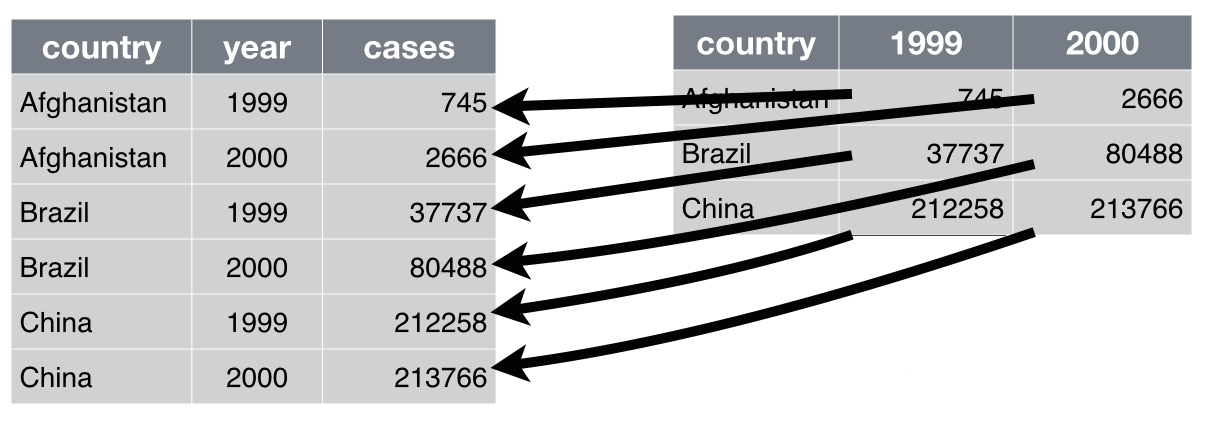
\includegraphics[width=\textwidth]{tidyr-gather.png}

{\footnotesize \href{http://garrettgman.github.io/tidying/}{Fuente}}
\end{center}
\end{frame}

\begin{frame}[fragile]
\frametitle{Ejemplo spread}
\begin{center}
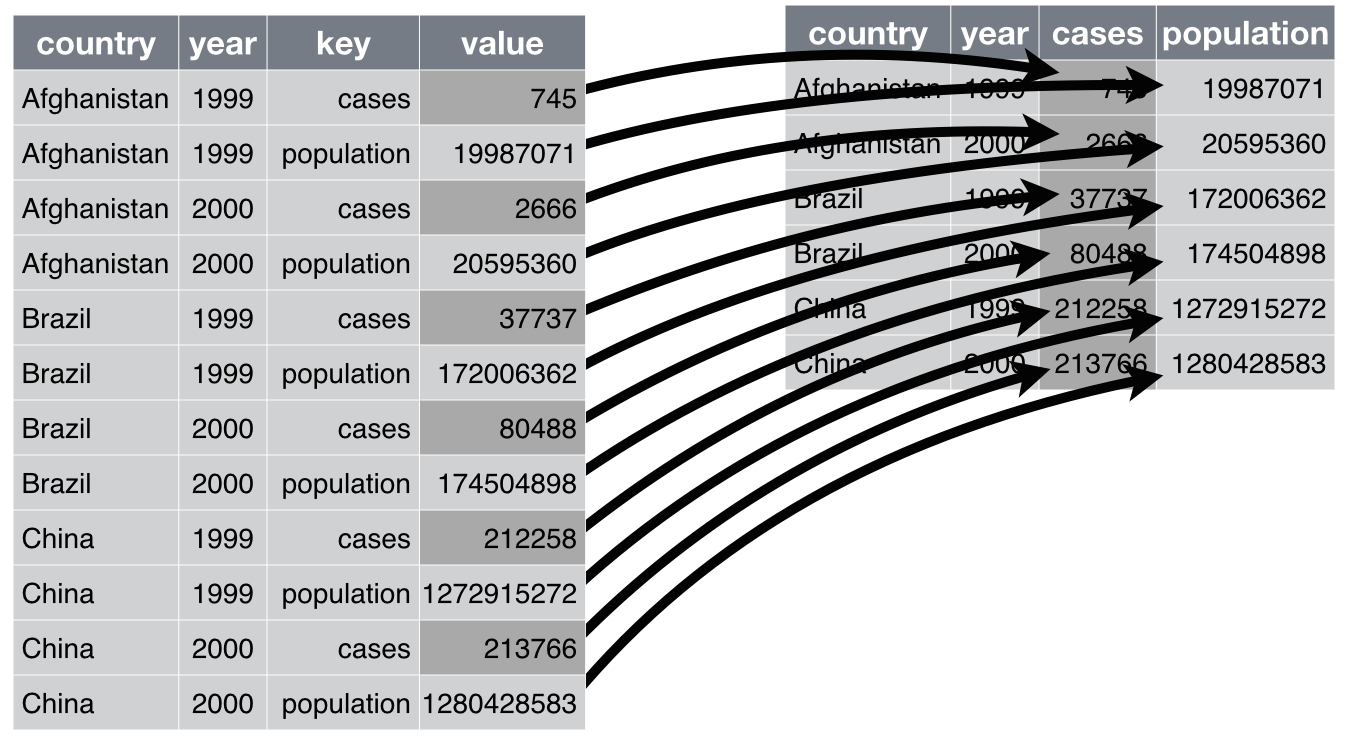
\includegraphics[width=\textwidth]{tidyr-spread.png}

{\footnotesize \href{http://garrettgman.github.io/tidying/}{Fuente}}
\end{center}
\end{frame}

%\begin{frame}
%\frametitle{Ejercicio ggplot2}
%
%Con el dataset \texttt{diamonds}, hacer un muestreo aleatorio de 100 puntos e intentar reproducir el gráfico:
%
%\centering
%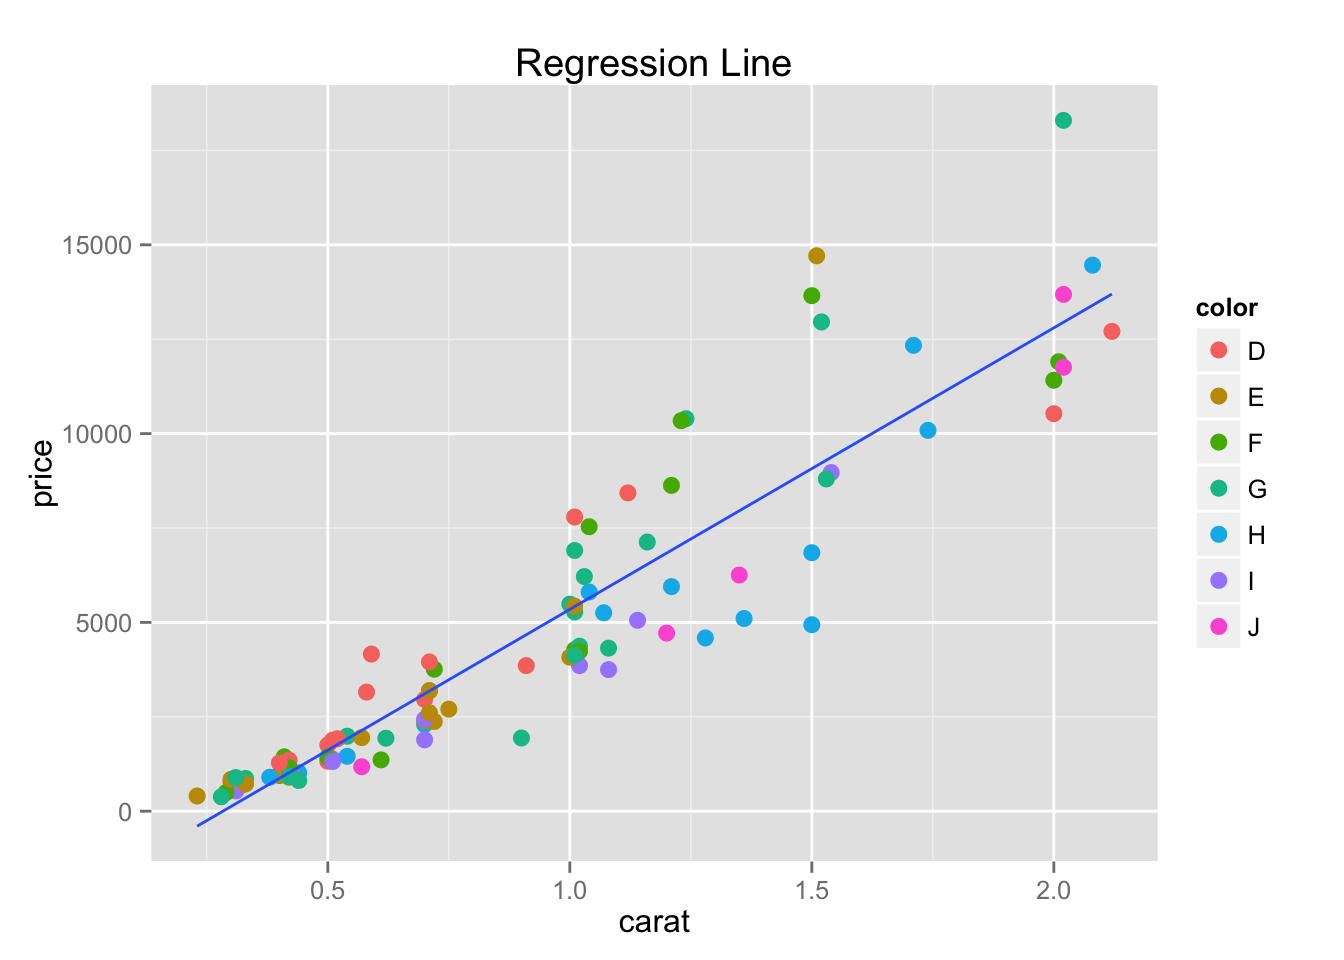
\includegraphics[width=0.9\textwidth]{ejercicio1.png}
%\end{frame}

\begin{frame}[fragile]
\frametitle{Paquete \texttt{readr}}

\begin{itemize}
\item Los datos suelen leerse desde archivos de texto externos.
\item La funciones principales del paquete \texttt{readr} son:
\begin{itemize}
\item \texttt{read\_delim()}, para ficheros separados por un delimitador
\item \texttt{read\_csv()}, para ficheros separados por comas
\end{itemize}
\item Ambos tienen un parámetro que es el nombre del fichero y devuelven un tibble.
\item Igual que en los scripts, el $fichero$ tiene que estar en el directorio de trabajo o en su defecto escribir la ruta completa.
\item Para escribir un data.frame o tibble en un fichero de texto se puede usar la función \texttt{write\_csv()}.
\end{itemize}

\end{frame}


\begin{frame}[allowframebreaks]
\frametitle{Parámetros opcionales}

Tiene los siguientes parámetros opcionales:
\begin{description}
\item[col\_names] Si TRUE, la primera fila es el nombre de las variables. También se le puede pasar un vector de cadenas de caracteres con los nombres.
\item[delim] Carácter que separa las columnas (solo en \texttt{read\_delim()}.
\item[na] Vector con cadenas que se interpretan como \textit{missing values}. Por defecto \texttt{"NA"} y la cadena vacía.
\item[col\_types] Vector de clases para las columnas (ver documentación de \texttt{col()}. Por defecto se intenta adivinar el tipo de cada columna a partir de las 1000 primeras líneas.
\framebreak
\item[n\_max] Número máximo de líneas a leer del fichero.
\item[skip] Número de líneas a ignorar al princpio del fichero.
\item[locale] Objeto que nos permite cambiar el enconding, separador decimal y formato de fechas. Ver documentación de \texttt{locale()}.
\item[comment] Una cadena de caracteres que identifica líneas de texto a ignorar (comentarios).
\item[trim\_ws] Si vale \texttt{TRUE}, se eliminan los espacios en blanco al principio y al final de cada campo.
\end{description}
\end{frame}


\begin{frame}
\frametitle{Otros formatos}
\begin{itemize}
\item Las funciones anteriores solo son capaces de leer ficheros de texto en los formatos más comunes.
\item Para otros formatos, existen paquetes específicos:
\begin{itemize}
\item \texttt{haven} para ficheros SPSS, Stata, y SAS.
\item \texttt{readxl} para ficheros de Excel (tanto .xls como .xlsx).
\item \texttt{DBI}, junto con otro paquete específico dependiendo del tipo de BD (por ejemplo \texttt{RMySQL}, \texttt{RSQLite}, \texttt{RPostgreSQL}, etc.) permite ejecutar \textit{querys} contra una base de datos, devolviendo un data.frame.
\item \texttt{jsonlite}, para ficheros JSON.
\item \texttt{xml2}, para ficheros XML.
\end{itemize}
\end{itemize}
\end{frame}


\begin{frame}
\frametitle{Ejercicio \texttt{ventas}}

\begin{itemize}
\item Cargar el conjunto de datos \texttt{ventas.csv} en R.
\item Ver que columnas tiene y su tipo.
\item Calcular la diferencia media en valor absoluto entre las ventas y su previsión.
\item Eliminar la variable \texttt{Prevision}.
\item Calcular la matriz de correlación de las \texttt{Ventas} para todos los distintos productos (identificados con su código).
\item Transformar la matriz de correlación anterior en un data.frame que esté en formato largo. Pista: identificar que variables deberían ir en las columnas.
\item Hacer un \textit{heatmap} que represente la matriz de correlación anterior. Pista: \texttt{geom\_tile}.
\end{itemize}
\end{frame}

\begin{frame}
\frametitle{Libros y manuales}

En general, se pueden encontrar muchos manuales en las secciones \textit{Manuals} y \textit{Contributed} de \href{https://cran.r-project.org/}{CRAN}, así como ejemplos en la web \href{https://rpubs.com/}{RPubs}. Algunos recursos más específicos:

\begin{description}
\item[Libros]
\begin{itemize}
 \item R for Data Science \href{http://r4ds.had.co.nz/}{[url]}.
 \item An Introduction to Statistical Learning with Applications in R \href{http://www-bcf.usc.edu/~gareth/ISL/}{[url]}.
\end{itemize}
\item[E-Books]
\begin{itemize}
\item YaRrr! The Pirate's Guide to R \href{http://nathanieldphillips.com/thepiratesguidetor/}{[url]}.
\item The R Inferno \href{http://www.burns-stat.com/pages/Tutor/R_inferno.pdf}{[url]}.
\item R Programming \href{https://en.wikibooks.org/wiki/R_Programming}{[url]}.
\end{itemize}
\item[Blogs]
\begin{itemize}
\item RTutorial \href{http://www.r-tutor.com/}{[url]}.
\item Quick-R \href{http://www.statmethods.net/}{[url]}.
\item RStudio \href{https://blog.rstudio.org/}{[url]}.
\item RBloggers \href{https://www.r-bloggers.com/}{[url]}.
\end{itemize}
\end{description}

\end{frame}

\begin{frame}
\frametitle{FAQ y comunidades}
\begin{itemize}
\item \href{http://stackoverflow.com/questions/tagged/r}{StackOverflow}: las preguntas con el tag R contienen mucha información y problemas resueltos. Además, las nuevas preguntas se responden en cuestión de horas.

\item \href{http://stats.stackexchange.com/}{CrossValidated}: no es una comunidad específica de R (más bien de estadística), pero hay mucha información acerca de cómo realizar procedimientos concretos de análisis de datos y aprendizaje automático en R.

\item \href{https://twitter.com/RLangTip}{@RLangTip}: Twitter que publica consejos y trucos diarios.

\item \href{https://plus.google.com/u/0/communities/115516770321395255377}{R Programming for Data Analysis}: Comunidad de Google+.
\item \href{https://plus.google.com/u/0/communities/117681470673972651781}{Statistics and R}: Otra comunidad de Google+.
\item \href{https://www.linkedin.com/grp/home?gid=77616}{The R Project for Statistical Computing}: Grupo de LinkedIn.
\end{itemize}
\end{frame}
\end{document}
